
%----------------------------------------------------------------------------
\chapter{Evaluation}
%----------------------------------------------------------------------------


\section{Measurement setup}

To measure the performance of the code generated by our framework we use the following setup.
We use 6 BeagleBone Black (BBB) \cite{BBB} as computing units. 
We connect them via network. 


\section{Measurement scenarios}

We generated models of size 45, 450, 4500, and 45000.

The models are partitioned to computing units in 3 different ways 
\begin{itemize}
	\item Standard -- The model is partitioned by equally distributing the model considering locality ie.\ elements that are connected have more probability of being allocated to the same unit
	\item Alternative -- It is the similar to the standard model, but trains are allocated to a single computing unit. Other elements are allocated to the other 5 computing units considering locality.
	\item Single -- All of the elements are allocated on the same computing unit
\end{itemize}

We measured on this 12 type of models 4 queries: \texttt{closeTrains}, \texttt{derailment}, \texttt{endOfSiding} and\texttt{trainLocations}. 
These were described in \autoref{sec:vql-examples}.

We used both of direct and interpreted code generation.
We measured the execution time of queries 10 times and took their average.

\section{Results, and evaluation}

The results of the measurements can be seen in \autoref{fig:measurement-int}, which shows how generating a search plan, and executing it by interpretation performed, and in \autoref{fig:measurement-dir}, which shows how direct code generation performed.

We can conclude, that direct code generation is more efficient for larger models than interpreting search plans at runtime. Interpreted search plans are faster for some smaller models only.

The performance for larger models is also independent of allocations. In case of direct code generation, \texttt{derailment} and \texttt{endOfSiding} queries were faster for smaller models. 
We examined the generated search plans for these patterns and found that these search plans checked whether the train is on the given segment at a later phase of execution, thus the train does not have to be on the same partition, as opposite reference is available at a \texttt{RailRoadElement}.

\pagebreak
\begin{figure}[H]
	\begin{center}
		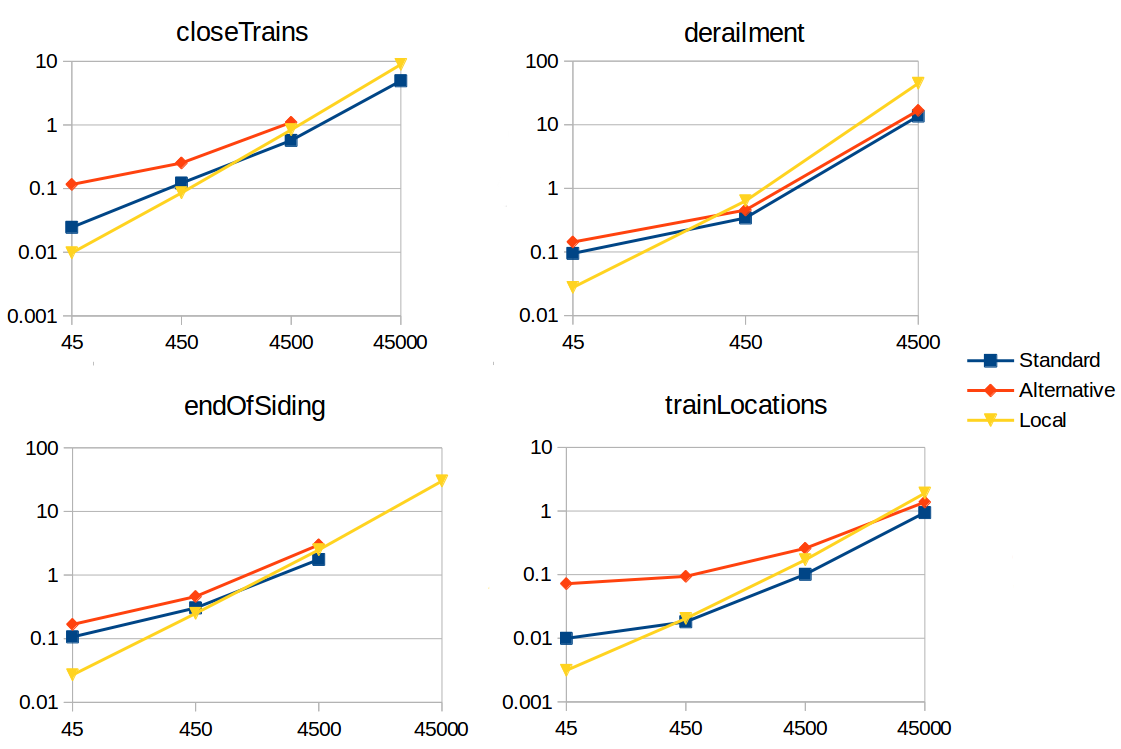
\includegraphics[width=\textwidth]{figures/measurement-interpreted-code.png}
		\caption{Results for interpreted search plan execution}
		\label{fig:measurement-int}
	\end{center}
\end{figure}

\begin{figure}[H]
	\begin{center}
		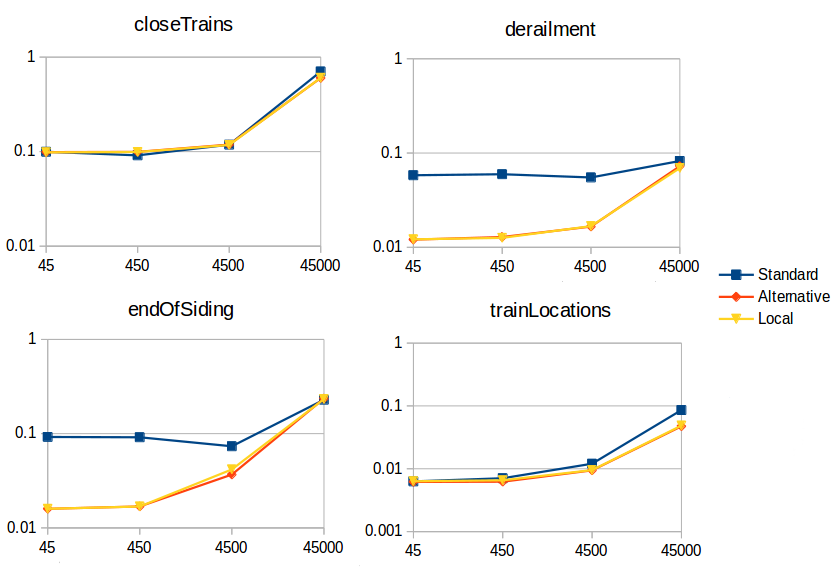
\includegraphics[width=\textwidth]{figures/measurement-directcode.png}
		\caption{Results for direct code generation}
		\label{fig:measurement-dir}
	\end{center}
\end{figure}


